\chapter{Architecture \& Design}

\emph{Status: Started}

\begin{figure}[ht]
    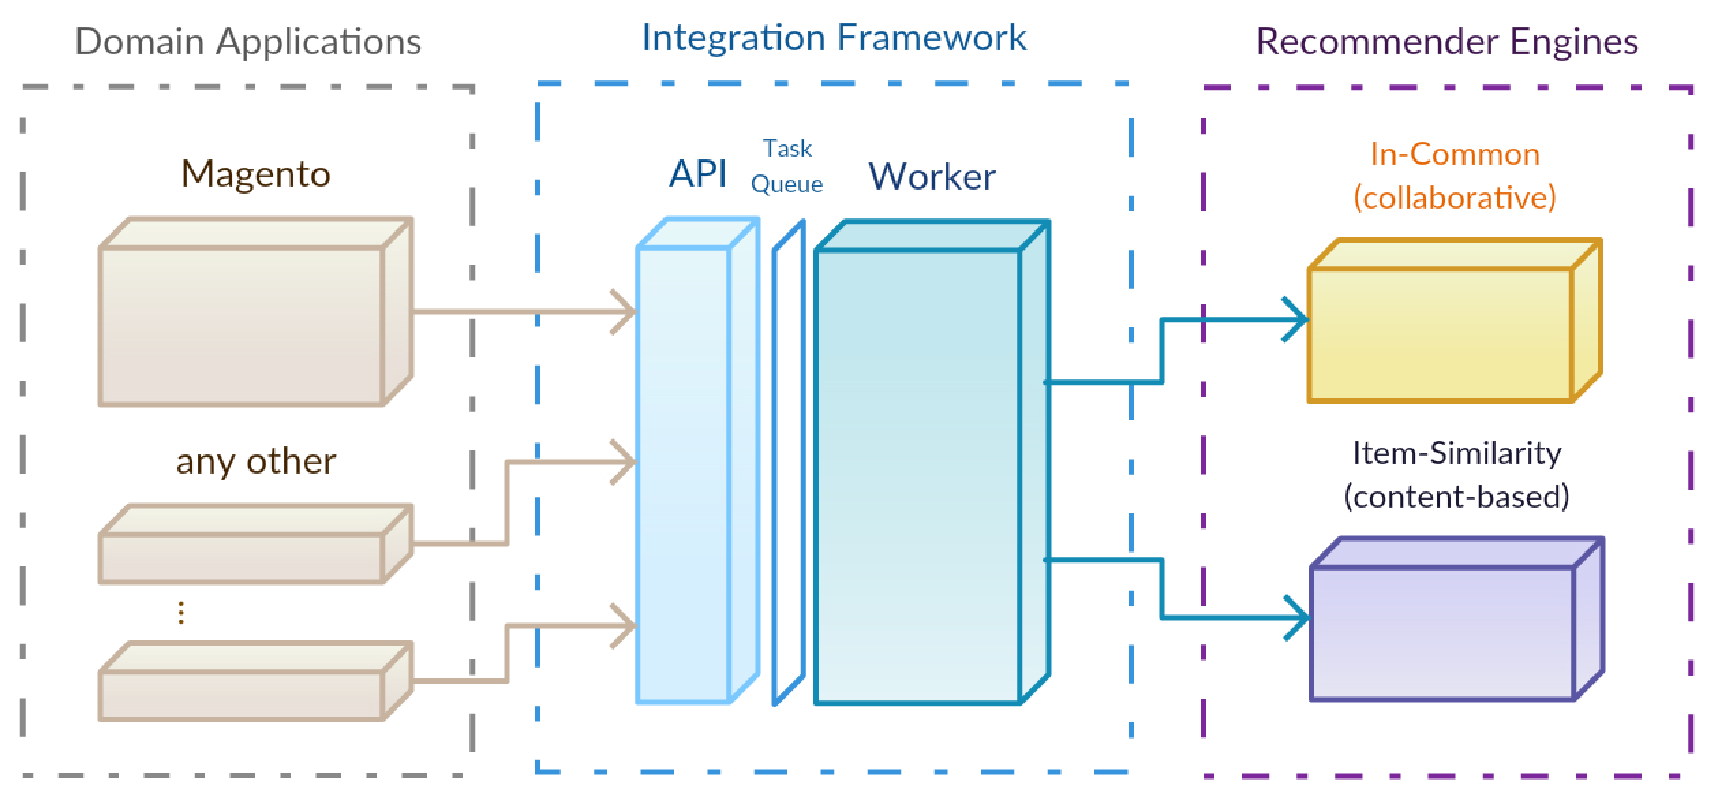
\includegraphics[width=\textwidth,center]{architecture/overview.pdf}
    \caption{Architectural Overview}
    \label{fig:architecture}
\end{figure}

\section{Domain Systems}
\label{architecture-domain-systems}

Throughout this report, \emph{domain systems} refer to existing systems primarily developed for a specific organisation or application, secondarily planning to make use of recommendations and integrate recommendation engines. The definition highlights the fact that these systems are usually built on extensive domain knowledge. Efforts to use recommendations either require domain savvy engineers to gain a recommendation background or recommendation savvy engineers to grasp the domain knowledge. The technology is mostly tailored to the requirements of those systems and may not be the first choice for recommendation requirements. A solution is therefore to develop these requirements as a separate system which is then integrated into the domain system. As explained in the introduction, this project provides a structured way of such integration. Figure \ref{fig:architecture} illustrates that this project supports the integration of as many domain systems as required in a single set-up.

Regarding knowledge, the proposed solution abstracts the internals of both domain and recommender systems. In order for the domain system to provide the requirements for the integration, knowledge about the internals of recommender systems is not required. In fact, to achieve interoperability -- as discussed in section \ref{intro-objectives-abstraction} -- recommender-specific approaches are not wished. For this reason, the emphasis of the integration on the domain systems side lies in the extraction of the data of interest for recommendations. Furthermore the terminology in this data can remain the same as used in the domain systems.

As far as the domain systems are concerned, keeping the integration effort and impact as minimal as possible was of much importance in this project. A typical negative impact of integrating systems is on performance; hence, the integration has been designed to minimise blocking on the domain systems. As a matter of fact, the number of required components which will be discussed in the next section has been decreased from proposed three -- \emph{Events}, \emph{Master Data} and \emph{Recommendation} -- to two with \emph{Master Data} being incorporated into \emph{Events}.

To conclude, this section has provided a definition for domain systems touching on some characteristics of their integration which shall be further detailed in the next sections.

\section{Framework}

\emph{Status: Not Started}

\begin{figure}[ht]
    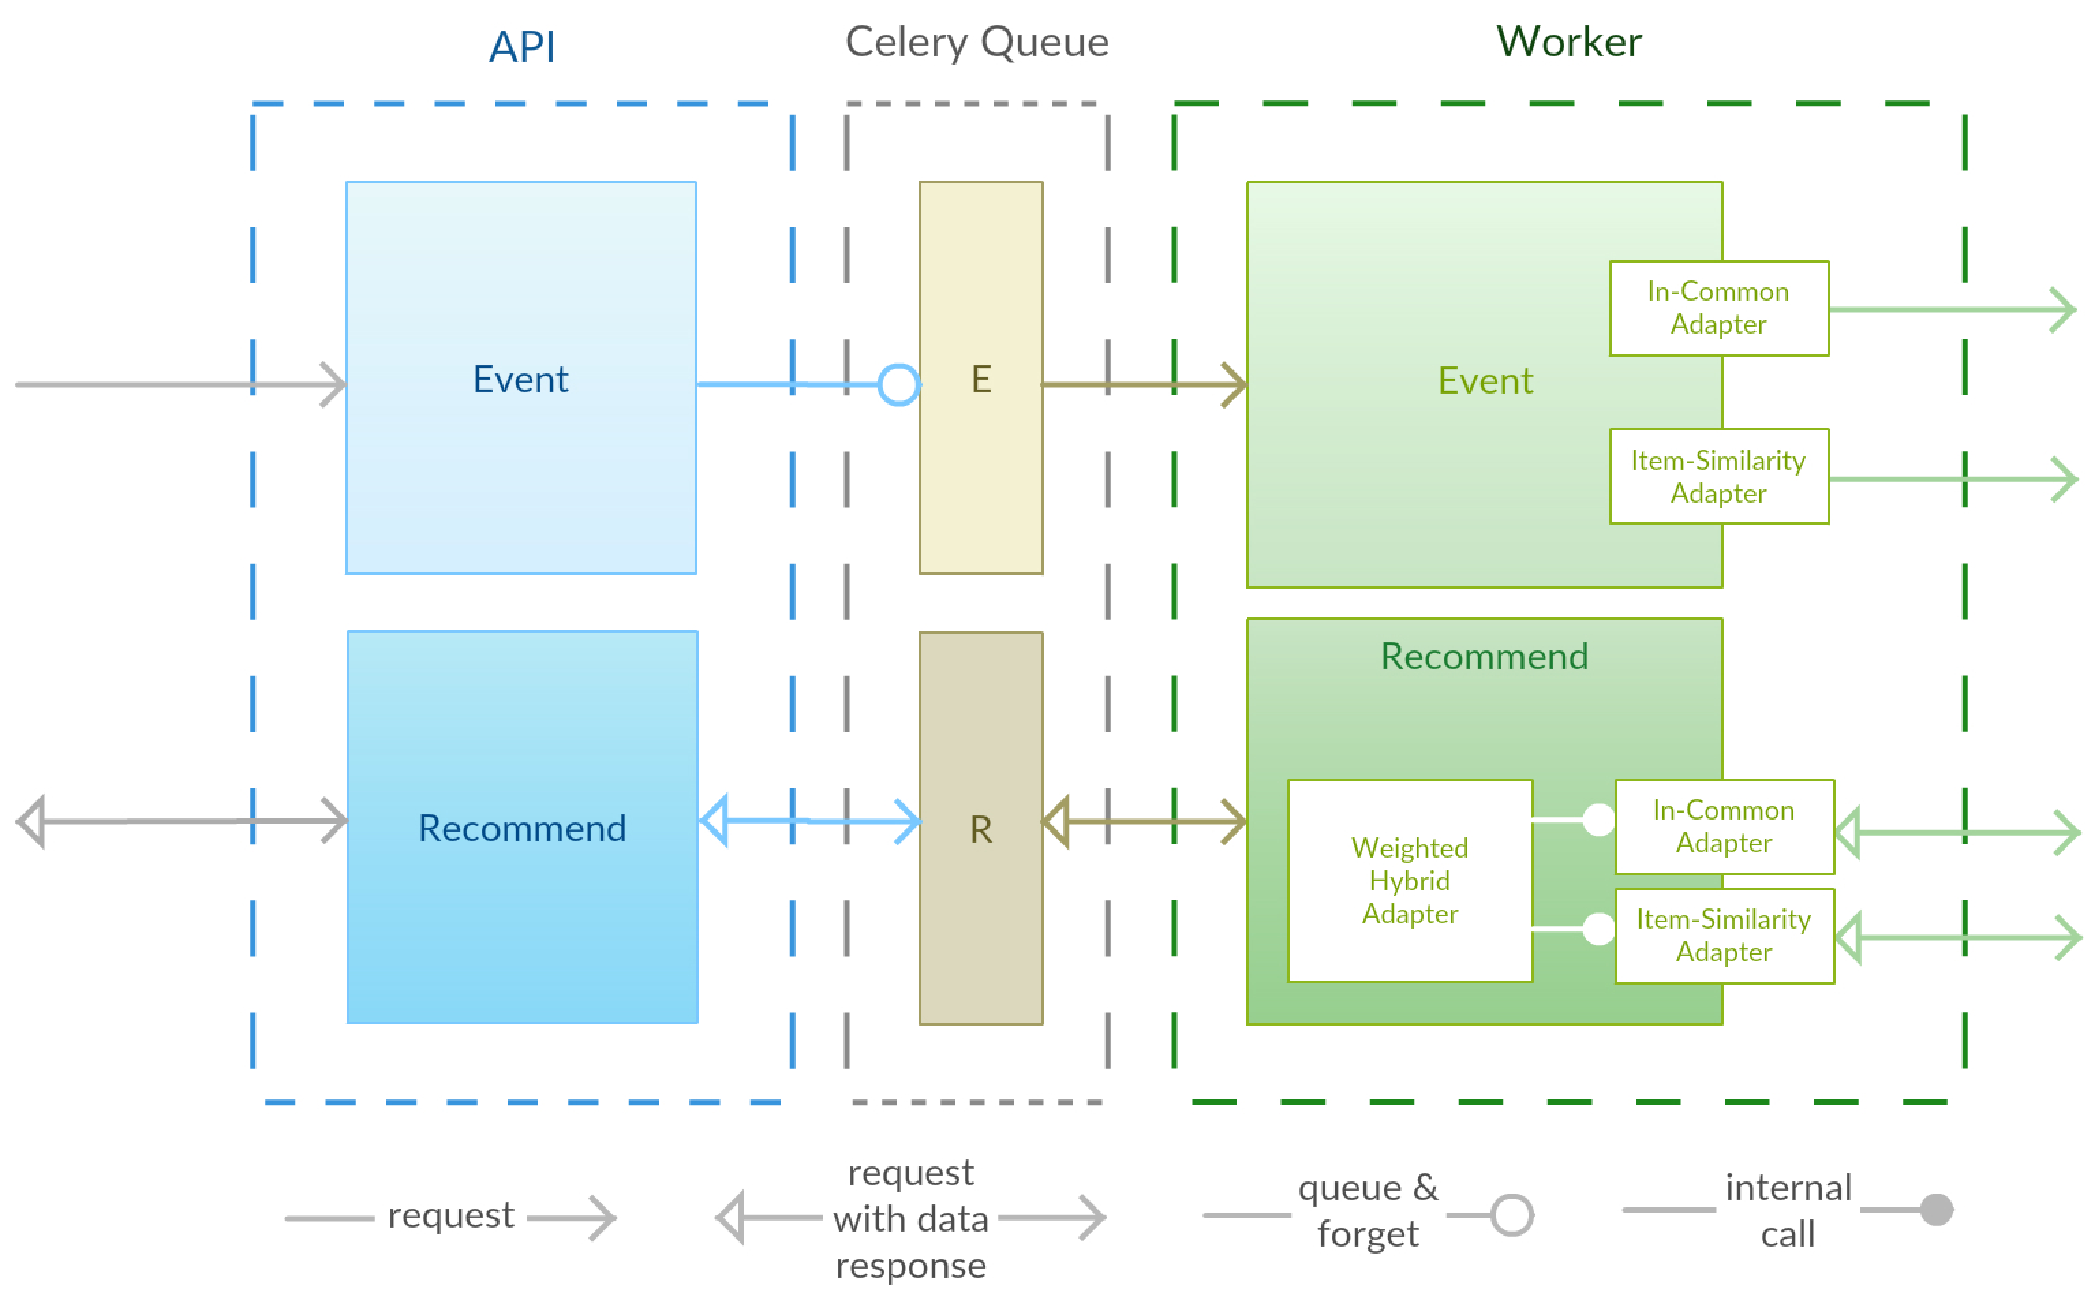
\includegraphics[width=\textwidth,center]{architecture/framework.pdf}
    \caption{Framework Design}
    \label{fig:collaborative}
\end{figure}

\begin{itemize}
\item Centrepiece of this work
\end{itemize}

\subsection{API}

\emph{Status: Not Started}

\begin{itemize}
\item No business
\end{itemize}

\subsection{Worker}

\emph{Status: Not Started}

\begin{itemize}
\item Holds business logic
\item Priority for recommendations
\item Can be spinned up as many as needed
\end{itemize}

\subsection{Concepts}

\emph{Status: Not Started}

\subsubsection{Events}

\emph{Status: Not Started}

\begin{itemize}
\item No master data specific logic, those are also treated as events
\end{itemize}

\subsubsection{Taxonomy}

\emph{Status: Not Started}

\subsubsection{Recommender}

\emph{Status: Not Started}

\subsubsection{Hybrid Recommender}

\emph{Status: Not Started}

\section{Engines}

\emph{Status: Not Started}

\begin{itemize}
\item Explain why separate from framework
\item Explain why no single layer and single storage
\item Enables to use the best technology incl. storage technology for the use-case
\item Enables to use existing recommender implementations in their technology stack
\item Requires a thin engine adapter in the framework
\end{itemize}

\subsection{Hybrid Recommender Engines}

\emph{Status: Not Started}